%=====================
\chapter{Requirements}
%=====================
\label{chap:req:requirements}
This chapter describes an utility that creates Wireshark dissectors from C
header files. The dissectors must interpret binary representations of C
structs. In \autoref{sec:req:list} we give a high level overview of the
utility and lists all the functional and non-function requirements.

\hyperref[sec:req:stories]{Section \ref*{sec:req:stories}} gives user stories
for the requirements, while \autoref{sec:req:usecases} provides use cases for
the utility, and \autoref{sec:prodbacklog} contains the complete product
backlog.

%-----------------------------
\section{List of requirements}
%-----------------------------
\label{sec:req:list}

\subsection{Overview}
%-----------------
We are to create an utility that allows Wireshark to interpret the binary
representations of C-language structs. While C structs seldom are exchanged
across networks, they are sometimes used in inter-process communication. The
purpose of the utility described here is to provide Wireshark with the
capability of automatically dissecting the binary representation of a C struct,
as long as its definition is known.

The expected work flow for the utility is to read one or more C header files,
which contain struct definitions, and output Wireshark dissectors, implemented
in Lua scripts. A configuration file or source code annotations in the header
files may be used when additional configuration is required.

\autoref{tab:req:func} lists the functional requirements, while
\autoref{tab:req:nonfunc} lists the non-functional requirements. Each
requirement have a priority (Pri) and a complexity (Cmp): High (H), 
Medium (M) or Low (L) which is explained in \autoref{sec:req:priority} and
\autoref{sec:req:compl}.

\subsection{Prioritization}
%--------------------------
\label{sec:req:priority}
The team has, in cooperation with the customer, prioritized the requirements
in three categories:
\begin{inparaenum}[\itshape a\upshape)]
	\item High,
	\item Medium or
	\item Low.
\end{inparaenum} 

\begin{description}
	\item[High] Core functionality of the utility which must be implemented.
	\item[Medium] Requirements that will improve the value of the utility.
	\item[Low] Requirements that will not add much value to the utility.
\end{description}

\subsection{Complexity}
%----------------------
\label{sec:req:compl}
The team has estimated the complexity for each requirement. We use the same
categories as for requirements priority:
\begin{inparaenum}[\itshape a\upshape)]
	\item High,
	\item Medium or
	\item Low.
\end{inparaenum} 

\begin{description}
	\item[High] Functionality which seems difficult and non-trivial to create.
	\item[Medium] Functionality that seems time consuming but straight forward.
	\item[Low] Requirements that are trivial to implement.
\end{description}

\begin{table}[htbp] \footnotesize \center
\caption{Functional Requirements\label{tab:req:func}}
\noindent\makebox[\textwidth]{%
\begin{tabularx}{1.2\textwidth}{l X c c}
	\toprule
	ID & Description & Pri. & Cmp. \\
	\midrule
	FR1 & The utility must be able to read basic C language struct definitions from C header files & H & \\
	FR1-A & The utility must support the following basic data types: int, float, char and boolean & H & L \\
	FR1-B & The utility must support members of type enum & H & L \\
	FR1-C & The utility must support members of type struct & H & M \\
	FR1-D & The utility must support members of type union & M & M \\
	FR1-E & The utility must support members of type array & H & M \\
	FR1-F & The utility should detect structs with the same name, and report it as an error & M & L \\
	\midrule
	FR2 & The utility must be able to generate Lua dissectors for Wireshark for the binary representation of C struct & H & \\
	FR2-A & The dissector shall be able to display simple structs & H & L \\
	FR2-B & The dissector shall be able to support structs within structs & M & M \\
	FR2-C & The dissector must support Wireshark's built-in filter and search on attributes & H & L \\
	FR2-D & The dissector shall be able to recognize invalid values for a struct member & L & L \\
	\midrule
	FR3 & The utility must support C preprocessor directives and macros & H & \\
	FR3-A & The utility shall support \#include & H & L \\
	FR3-B & The utility shall support \#define and \#if & H & L \\
	FR3-C & The utility shall support \verb+WIN32+, \verb+_WIN32+, \verb+_WIN64+, \verb+__sparc__+, \verb+__sparc+ and \verb+sun+ & M & H \\
	\midrule
	FR4 & The utility must support user configuration & M & \\
	FR4-A & Configuration must support valid ranges for struct members & L & L \\
	FR4-B & Configuration must support custom Lua files for specific protocols & H & H \\
	FR4-C & Configuration must support custom handling of specific data types & L & M \\
	FR4-D & Configuration must support specifying the ID of dissectors & H & L \\
	FR4-E & Configuration must support various trailers (other registered protocol) & L & H \\
	FR4-F & Configuration must support integer members which represent enumerated named value & M & L \\	
	FR4-G & Configuration must support members which are bit string & M & L \\
	\midrule
	FR5 & The dissectors must be able to handle binary input which size and endian depends on originating platform & M & \\
	FR5-A & Flags must be specified in configuration for each platform & M & M \\
	FR5-B & Flags within message headers should signal the platform & M & H \\
	FR5-C & Generate dissectors which support both little and big endian platforms & H & M \\
	FR5-D & Generate dissectors which support different sizes depending on platforms & M & H \\
	\midrule
	FR6 & The utility shall support parameters from command line & H & \\
	FR6-A & Command line shall support parameters for C header file & H & L \\
	FR6-B & Command line shall support for configuration file & H & L \\
	FR6-C & Command line shall support batch mode of C header and configuration files & L & M \\
	FR6-D & When running batch mode, dissectors that already are generated, shall not be regenerated, if the source are not modified since last run & L & M \\
	\bottomrule
\end{tabularx}}
\end{table}

\begin{table}[htbp] \footnotesize \center
\caption{Non-Functional Requirements\label{tab:req:nonfunc}}
\noindent\makebox[\textwidth]{%
\begin{tabularx}{1.2\textwidth}{l X c c}
	\toprule
	ID & Description & Pri. & Cmp. \\
	\midrule
	NR1 & The utility shall be able to run on latest Windows and Solaris operating system & M & L \\
	\addlinespace
	NR2 & The dissector shall be able to run on Windows x86, Windows x86-64, Solaris x86, Solaris x86-64 and Solaris SPARC & M & M \\
	\addlinespace
	NR3 & The utility shall only have a command line user interface. No GUI \& clicking! & H & L \\
	\addlinespace
	NR4 & The utility must have sufficient documentation to allow a person, with no previous knowledge of the system or Wireshark, to be able to use it to generate Lua dissectors after 5 hours of reading & M & M \\
	\addlinespace
	NR5 & The utility must have sufficient documentation to allow a person, already proficient with the system, to be able to extend its functionality after Y hours of reading & M & M \\
	\addlinespace
	NR6 & The utility code should follow standard python coding convention as specified by PEP8 and try to follow python style guidelines defined by PEP20 & H & L \\
	\addlinespace
	NR7 & All Python modules, classes, functions and methods in the utility should have docstrings which explains their code & L & L \\
	\bottomrule
\end{tabularx}}
\end{table}


%---------------------
\section{User Stories}
%---------------------
\label{sec:req:stories}
This sections shows the user stories, these are display in
\autoref{tab:req:stories1} and \autoref{tab:req:stories2}. The developer in
this context is the developers at Thales Norway AS. The administrator is this
context is the users of the dissectors.

\begin{table}[htbp] \footnotesize \center
\caption{User stories part 1\label{tab:req:stories1}}
\noindent\makebox[\textwidth]{%
\begin{tabularx}{1.2\textwidth}{l X}
	\toprule
	Header. & Value \\
	\midrule
	ID:			& US01 \\
	Requirements:	& FR7-A: Command line shall support parameters for C-header file. \\
	Who:			&  Developer\\
	What:		&  The user wants the utility to generate a dissector from a C-header file that he specifies.\\
	How:			&  The command line user interface will accept a number of arguments from the user, one of which
				includes the path to an existing C header file and sends this to the parser module. It will parse these 
				arguments with the help of argparse library, which supports optional and positional arguments etc.\\
	Result:		& The command line interface supports C-headers as input. \\
	\midrule
	ID:			& US02 \\
	Requirements:	& FR1-A: The utility should support the following basic data types: int, float, char and boolean. \\
	Who:			&  Developer\\
	What:		&  The user wants the utility to support structs with members of basic data types in input files. 
					These are the basic data types in C which we support: int, float, char and boolean.\\
	How:			& The C parser library, pycparser, provides this support for us. In the cparser module we feed the
				 input into it, and then extracts the definitions from an abstract syntax tree which it generates for us.  \\
	Result:		& The utility supports input with C structs with int, float, char and boolean members. \\
	\midrule
	ID:			& US03 \\
	Requirements:	& FR3-A: The utility should support \#include.\\
	Who:			& Developer \\
	What:		&  The user wants the utility to support the \#include-statement inside a header file.\\
	How:			& The cparser module feeds the input into an external tool, the C preprocessor, which supports 
				\#include-statements. It returns a C code file with all the included code from the external files. pycparser
				 provides support using a C-preprocessor.  \\
	Result:		& The utility supports \#include. \\
	\midrule
	ID:			& US04 \\
	Requirements:	& FR3-B: The utility should support \#define and \#if. \\
	Who:			&  Developer\\
	What:		&  The user wants the utility to support \#define- and \#if-statement inside a header file.\\
	How:			& The cparser module feeds the input into an external tool, the C preprocessor, which supports 
				\#define- and \#if-statements. It returns a copy of the file with the statements removed, and their actions performed. \\
	Result:		& The utility supports \#define and \#if functionality. \\
	\bottomrule
\end{tabularx}}
\end{table}

\begin{table}[htbp] \footnotesize \center
\caption{User stories part 2\label{tab:req:stories2}}
\noindent\makebox[\textwidth]{%
\begin{tabularx}{1.2\textwidth}{l X}
	\toprule
	Header. & Value \\
	\midrule
	ID:			& US05 \\
	Requirements:	&  FR2-D: Recognize invalid values for a struct member. \\
	Who:			& Administrator\\
	What:		& The user wants Wireshark to give a warning if a struct contains invalid values. \\
	How:			& The generated dissectors contain valid ranges for certain fields, and lua code which adds warning flags 
				in Wireshark if a specific fields value is outside the range. Wireshark color the display tree yellow to alert the 
				user of the error. The range is specified by configuration files. \\
	Result:		& The user can see when a value is out of range. \\
	\midrule
	ID:			& US06 \\
	Requirements:	& FR4-A: Configuration must support valid ranges for struct members. \\
	Who:			& Developer \\
	What:		& The user wants to be able to specify valid ranges for struct members in a configuration file. \\
	How:			& The config module should read config files provided to the command line interface, and find any rules 
				regarding valid ranges. The rules are used by the cparser when it translates struct definitions to Protocol 
				and Field instances found in the dissector module. \\
	Result:		&  \\
	\midrule
	ID:			& US07 \\
	Requirements:	&  FR7-B: Command line shall have support for configuration file(s). \\
	Who:			& Developer \\
	What:		& The user wants to provide the utility with one ore more configuration files. \\
	How:			& The command line interface should accept arguments which specifies the path of existing configuration
				 files, and feed these to the config module, which should read the files and store them in configuration data 
				 structures. These data structures will be available to cparser to help when translating structs to Protocol and
				  Fields from the dissector module. \\
	Result:		&  Configuration files can be input for the command line.\\
	\midrule
	ID:			& US08 \\
	Requirements:	&  FR2-A: The utility shall be able to display simple structs. \\
	Who:			& Administrator\\
	What:		& The user wants Wireshark to display simple structs. \\
	How:			& The dissector module shall generate Lua dissectors for Protocols created by the cparser module. 
				The Lua dissectors shall use Wireshark's API to display structs with basic members. \\
	Result:		&  \\

	\bottomrule
\end{tabularx}}
\end{table}


%------------------
\section{Use Cases}
%------------------
\label{sec:req:usecases}
This sections contains use case diagrams for our two actors, and detailed
textual use cases for these diagrams.

\subsection{Actors}
%------------------
An actor specifies a role played by an external person or thing that interact
with our utility. We have three types of actors to consider. First is the
primary actor which in our case is the user of our utility. He who feeds it a
C file to generate dissectors. A secondary actor is someone who configures our
utility to change the output of it. Finally we have an offstage actor which
does not use our utility himself, but uses the output dissectors in Wireshark.

We have defined two use case actors for our utility. The customer has specified
that the offstage actor, called administrator, is the most important actor.
\begin{description}
	\item[Administrator] User of the generated Wireshark dissectors, offstage actor
	\item[Developer] User and configurer of utility, primary and secondary actor
\end{description}

\subsection{Use Case Diagrams}
%-----------------------------
\hyperref[fig:req:ucadm]{Figure \ref*{fig:req:ucadm}} shows the use case
diagram for the administrator, and \autoref{fig:req:ucdev} is the use case
diagram for the developer.x
\begin{figure}[htbp]
	\center
	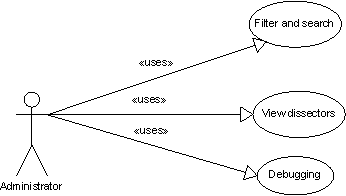
\includegraphics[width=0.8\textwidth]{./planning/img/administrator.png}
	\caption{Use Case Diagram: Administrator\label{fig:req:ucadm}}
\end{figure}

\begin{figure}[htbp]
	\center
	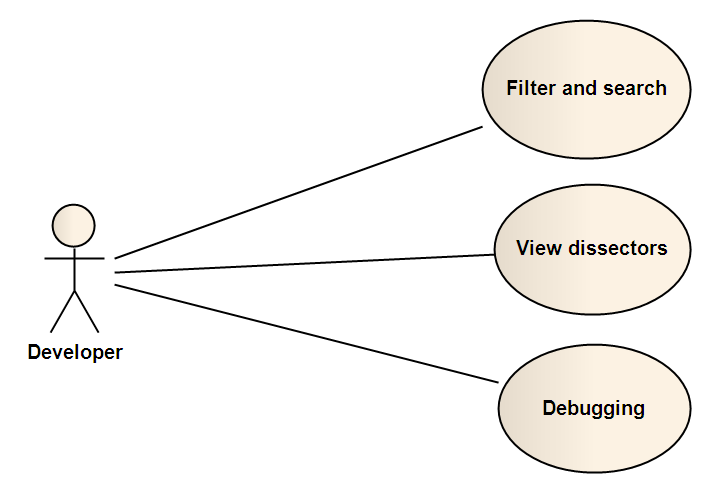
\includegraphics[width=0.8\textwidth]{./planning/img/developer.png}
	\caption{Use Case Diagram: Developer\label{fig:req:ucdev}}
\end{figure}

%Removed for pre-delivery
%\subsection{Textual Use Cases}
%-----------------------------
%TODO!!!

